\documentclass[a4paper,11pt]{scrartcl}
\usepackage{fullpage}
\usepackage[utf8]{inputenc}
\usepackage[english]{babel}
\usepackage{amssymb}
\usepackage{amsmath}
\usepackage{amsthm}
\usepackage{listings}
\usepackage{graphicx}
\usepackage{cite}

\usepackage[usenames,dvipsnames]{pstricks}
\usepackage{epsfig}
\usepackage{pst-grad} % For gradients
\usepackage{pst-plot} % For axes

\title{Seminararbeit Numerik}
\subtitle{Iterative Solvers - Algebraic Multigrid}
\author{Bernd Schwarzenbacher, Daniel Herold}

\begin{document}
\maketitle
\tableofcontents
\pagebreak

\section{Motivation} \label{section:motiv}
To solve big systems of linear equations the conjugate gradient method is the
most used iterative method. For faster convergence speed the condition of the
problem is further improved with a so-called preconditioner.
The original problem is therefore substituted by the preconditioned problem:
$$b-Ax = 0 \iff x + \tau C^{-1} (b-Ax) = x$$
Where the matrix $C$ denotes the preconditioner.

The Algebraic Multigrid (AMG) method combines several bad preconditioners to
obtain a good preconditioner in total. It belongs to the family of general
Multigrid (MG) methods which recursively coarsen the original matrix and
project the problem on this coarser spaces by use of a prolongation matrix.
On the coarser levels, low frequency errors in the solution are corrected
faster. The AMG method uses only the information in the system matrix to
compute the coarsening and further the projection matrix. It does so by
weighting the relative strength of connecting vertices to determine which
vertices should collapse on the next level.
\cite{numerik} \cite{numpde}

In the application of the AMG preconditioner we use one forward and one
backward Gauß-Seidel preconditioner per level. Additionally a
transposed matrix vector multiplication is needed to project onto the
coarse space. See Listing~\ref{lst:mult} for more details on the algorithm.
Those three points are subject to performance improvements by parallelization.

\section{Sparse Matrices}
Most matrices are stored in the Compressed Column Storage (CCS) format.
The commands {\em firsti[k]}\/ and {\em lasti[k]}\/ provide the position of the
first and last entry of the row k in the index vector. One
iteration through one row is very easy to provide.

\lstset{language=C++, numbers=none, captionpos=b,
        caption={Row-iteration of sparsematrices }}
\begin{lstlisting}
for (int j = firsti[k]; j < lasti[k]; ++j)
  {...}
\end{lstlisting}

The difficulty with sparse matrices is the iteration among any other order as
the next section will show.

\section{Matrix Vector Multiplication}
The multiplication of a sparse matrix and a given vector is very simple.
The entry k of the output vector is given by the summation of the products
of the matrix entries in the row k with the entries of the vector. In other
words, one entry of the output vector depends only on one row of the matrix
and vice versa.

One of the difficulties of parallelization is given by multiple writing
performances on a single variable at the same time. In the case of a simple
matrix vector multiplication this is no big deal to handle: each row has to be
executed by a single thread, there is no limitation in which order which thread
calculates its vector entry.

\lstset{language=C++, numbers=left, captionpos=b,
        caption={Matrix vector multiplication with parallel for section.}}
\begin{lstlisting}
void MultAddParallel w(double s, const BaseVector & x, BaseVector & y)
{
#pragma omp parallel for
    for (int i = 0; i < this->Height(); ++i) {
      int first = firsti [i];
      int last  = firsti [i+1];

      for (int j = first; j < last; ++j) {
        y(i) += s * data[j] * x(colnr[j]);
      }
    }
  }

\end{lstlisting}

\subsection{Transposed Matrix Vector Multiplication}\label{section:trans}
To provide the multiplication of a vector with the transposed matrix, a
sequential algorithm is written in a similar way.

\lstset{language=C++, numbers=none, captionpos=b,
        caption={Transposed vector multiplication algorithm.}}
\begin{lstlisting}
    for (int i = 0; i < this->Height(); ++i) {
      int first = firsti [i];
      int last  = firsti [i+1];

      for (int j = first; j < last; ++j) {
        y(colnr[j]) += s * data[j] * x(i);
      }
    }
\end{lstlisting}

The difference to the previous algorithm is due to the dependencies of a single
output vector entry. It is calculated by iterating through the entries
of one matrix column. This is not efficient due to the CCS format.
Therefore the algorithm has to iterate first through the matrix rows.
The access of distinct entries per row is no problem for the sequential
code, but simple parallelization causes issues.
Concurrent reading and writing operations to one variable can lead to incorrect
stored values as shown in figure~\ref{figure:parallelwriting}. Two
thread are trying to write at the same variable at almost the same time. The
second thread starts his procedure before thread 1 has finished and overwrites the
result of the first thread.

\begin{figure}[ht]
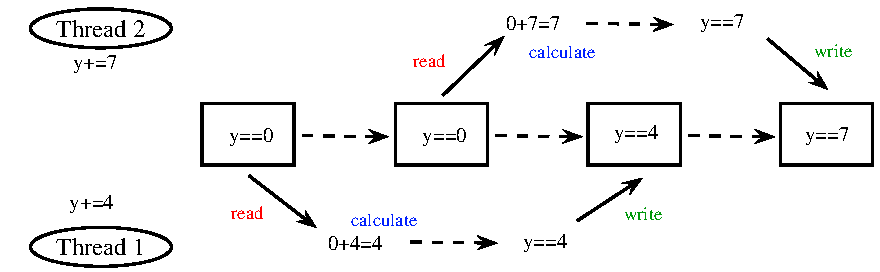
\includegraphics{graphic/parallel_writing_problem.pdf}
\caption{Problem with Parallelization of Writing Processes}\label{figure:parallelwriting}
\end{figure}

\begin{samepage}
Some ideas to solve this problem are:
\begin{itemize}
\item atomic writing process (easy to program, but very inefficient)
\item atomic writing process with dynamic thread partitioning
\item atomic writing process with static thread separation
\item matrix coloring without any atomic processes
\end{itemize}
\end{samepage}

All those solutions efficiency depend on the number of entries in the matrix.
Less entries and a larger matrix result in higher amounts of calculations per
time and thus are suited for parallel algorithms.
Whereas a sequential algorithm fares better than a parallel solution for
matrices with a high amount of nonzero elements for this problem.

The \textbf{atomic} version is very straight forward. The idea is to avoid the
problem shown in figure~\ref{figure:parallelwriting} by making the operations
atomic. This means that a thread blocks the address it accesses till it is
finished with its read-modify-write operation.

\lstset{language=C++, numbers=none, captionpos=b,
        caption={Atomic section in the transposed vector multiplication.}}
\begin{lstlisting}
#pragma omp atomic
          fy(colnr[j]) += s * data[j] * fx(i);
\end{lstlisting}

This part is the bottleneck of the algorithm, because every thread has to has
pass this line and they block each other.

The \textbf{dynamic thread partitioning} solves another problem of this code.
{\em OMP for}\/ (as used in the atomic version) splits the for-loop into a
evenly distributed amount of iterations for each thread beforehand. Due to
differing amount of calculations each thread has to perform, some may finish
faster than other thread. This relates to the specific structure of matrices
resulting in a finite element discretization, the number of nonzero elements
per row can vary significantly.

Instead it is possible to split the jobs dynamically. Faster threads are
assigned new iterations while slower thread still work on the old iterations.
The dynamic assignment produces some overhead, which can be mitigated by
assigning chunks of iterations.

\lstset{language=C++, numbers=none, captionpos=b,
        caption={Dynamic for loop.}}
\begin{lstlisting}
#pragma omp for schedule (dynamic, 100)
\end{lstlisting}

The \textbf{balancing option} performs a similar assignment of iterations, but
does so before the for-loop starts instead of a dynamic assignment. The work
for the calculation of each row is approximated with the number of nonzero
elements in this row and split the loop accordingly.

\lstset{language=C++, numbers=left, captionpos=b,
        caption={Static balancing in the transposed vector multiplication.}}
\begin{lstlisting}
void TranMultBalance (double s, const BaseVector & x, BaseVector & y) const
  {
    FlatVector<double> fx = x.FV<double> ();
    FlatVector<double> fy = y.FV<double> ();

    int height = this->Height();

    Array<int> thread_separation;
#pragma omp parallel //shared(thread_separation)
    {
      int num_threads = omp_get_num_threads();

#pragma omp single
      {
        thread_separation = Array<int>(num_threads+1);
        int separation_step = ceil(this->nze / num_threads);

        int thread_i = 1;
        for (int row = 0; row < height; ++row)
        {
          if (firsti[row] >= thread_i * separation_step)
          {
            thread_separation[thread_i] = row;
            ++thread_i;
          }
        }
        thread_separation[0] = 0;
        thread_separation[num_threads] = height;
      }

#pragma omp for
      for (int thread_i = 1; thread_i <= num_threads; ++thread_i)
      {
        for (int i = thread_separation[thread_i-1];
             i < thread_separation[thread_i]; ++i)
        {
          int first = firsti [i];
          int last  = firsti [i+1];

          for (int j = first; j < last; ++j)
          {
#pragma omp atomic
            fy(colnr[j]) += s * data[j] * fx(i);
          }
        }
      }
    }
  }

\end{lstlisting}

Every method still has the same problem with the atomic operation in its
essential part. We can avoid this by "\textbf{coloring}" each row of the matrix.
Rows are assigned to the same color if they don't write on the same entries.
Parallelization of this group is therefore possible, as no conflicting
concurrent operations will occur. Thus it is possible to iterate through the
colors sequentially and parallelize each color.

Not writing at the same entry is equivalent to not sharing any columns with
nonzero elements. Figure~\ref{figure:coloring} shows an example of the
coloring process.


\begin{figure}[ht]
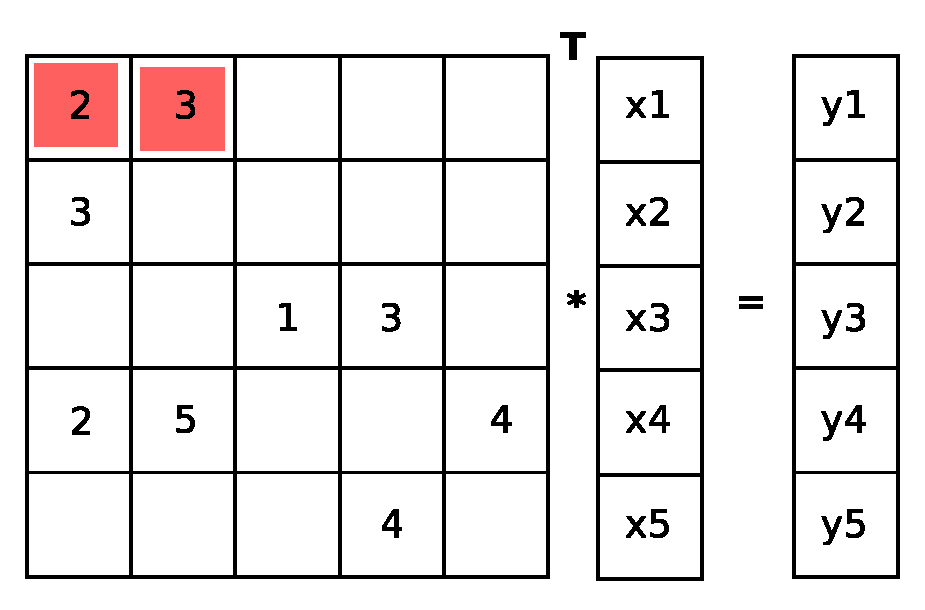
\includegraphics[width=0.32\textwidth]{graphic/coloringT2.eps}\hfill\vline\hfill
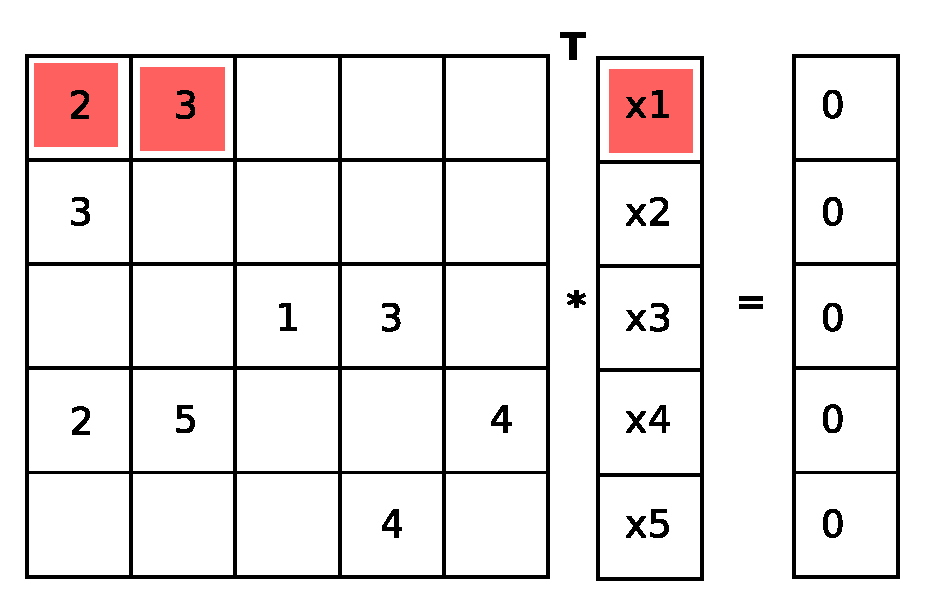
\includegraphics[width=0.32\textwidth]{graphic/coloringT3.eps}\hfill\vline\hfill
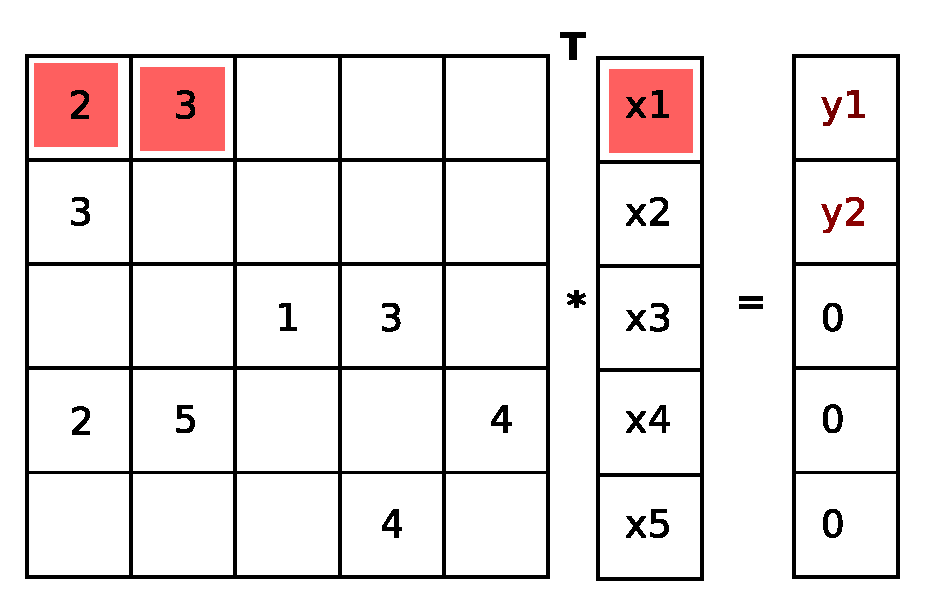
\includegraphics[width=0.32\textwidth]{graphic/coloringT4.eps}
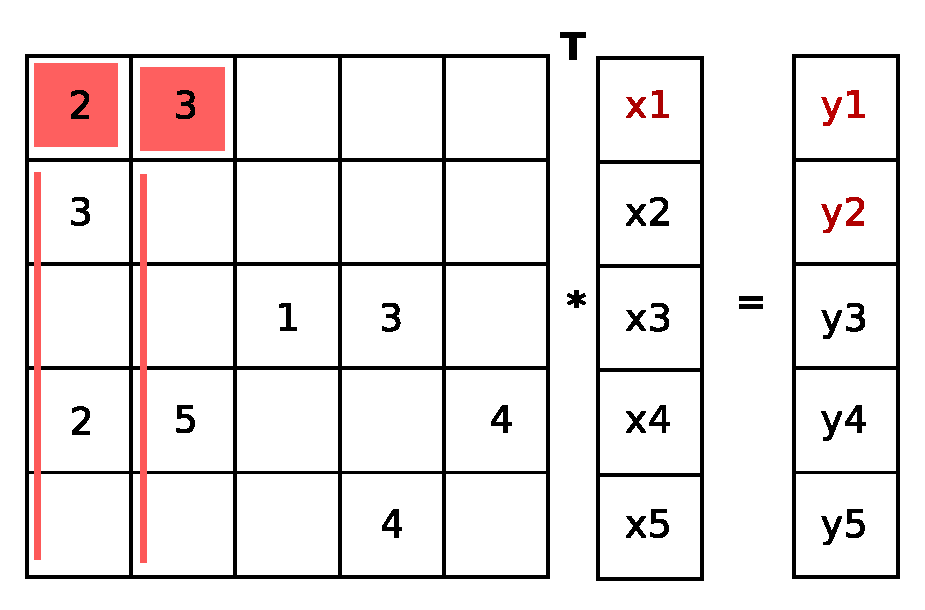
\includegraphics[width=0.32\textwidth]{graphic/coloringT5.eps}\hfill\vline\hfill
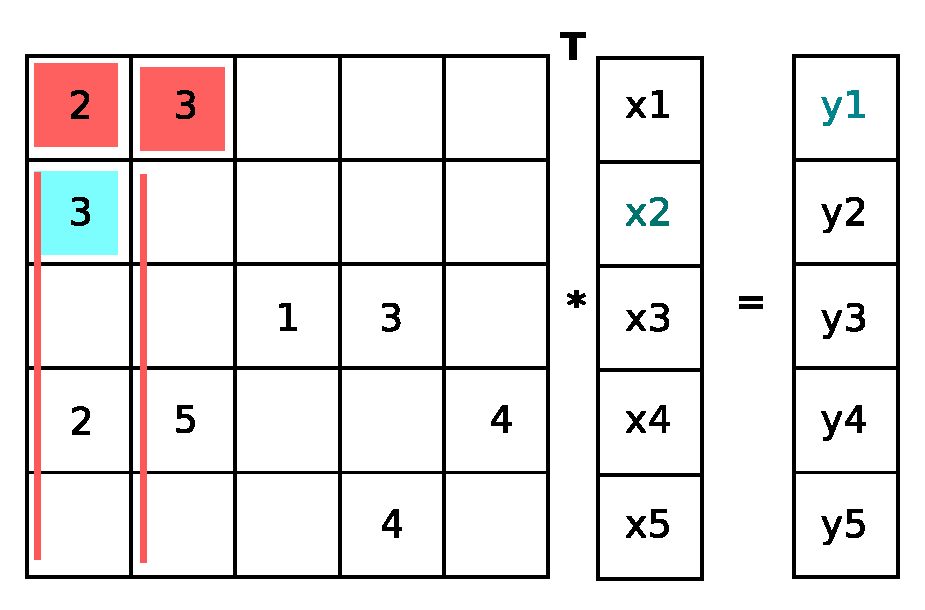
\includegraphics[width=0.32\textwidth]{graphic/coloringT6.eps}\hfill\vline\hfill
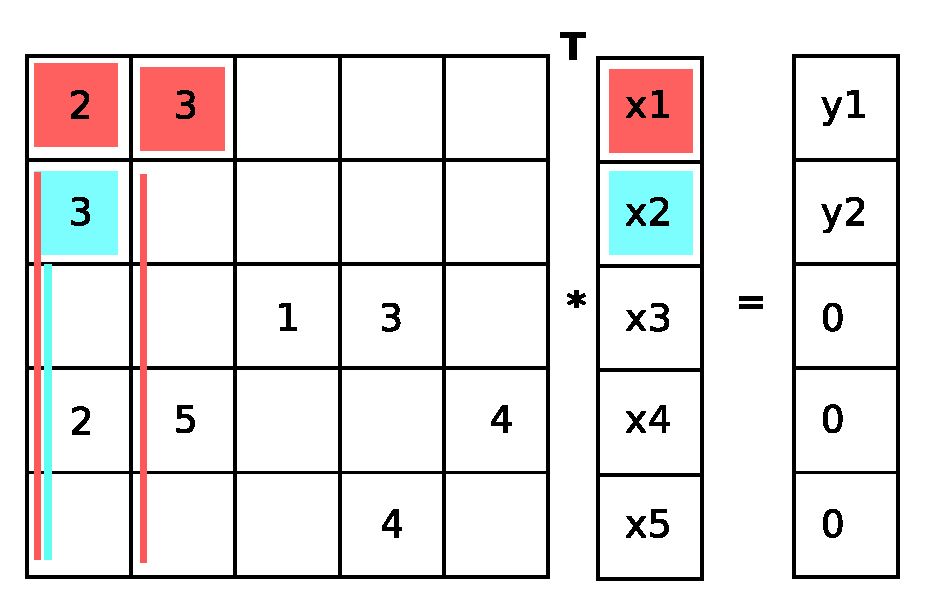
\includegraphics[width=0.32\textwidth]{graphic/coloringT7.eps}
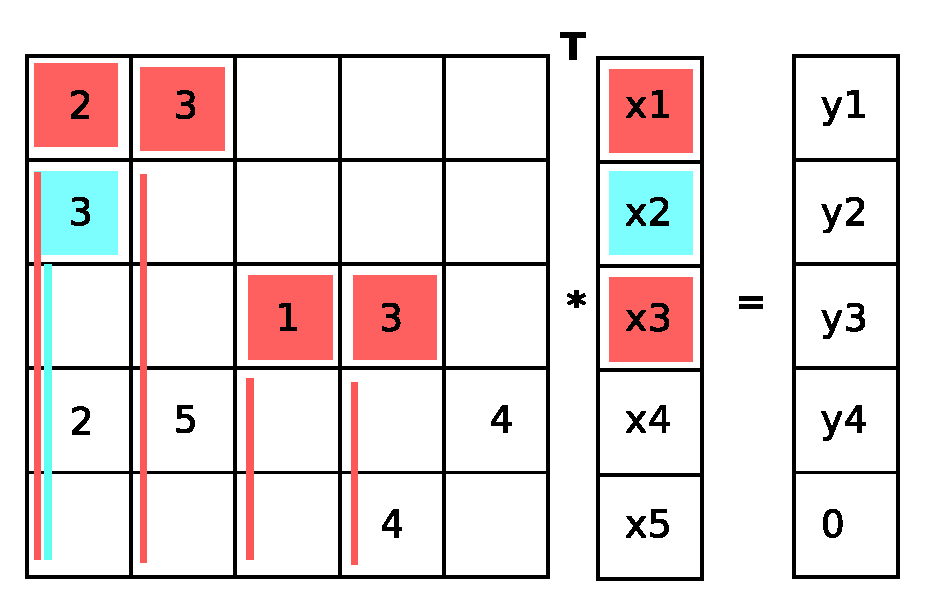
\includegraphics[width=0.32\textwidth]{graphic/coloringT8.eps}\hfill\vline\hfill
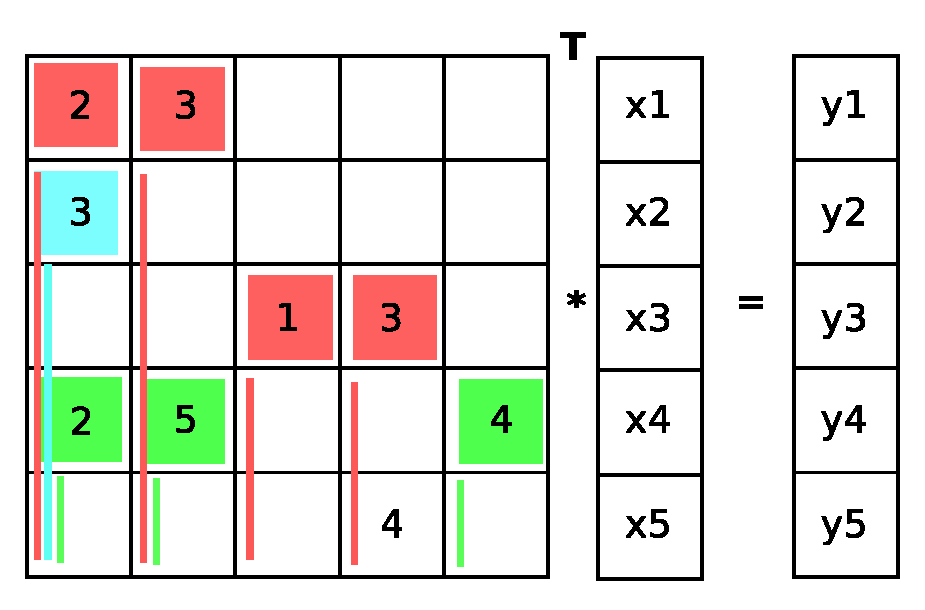
\includegraphics[width=0.32\textwidth]{graphic/coloringT9.eps}\hfill\vline\hfill
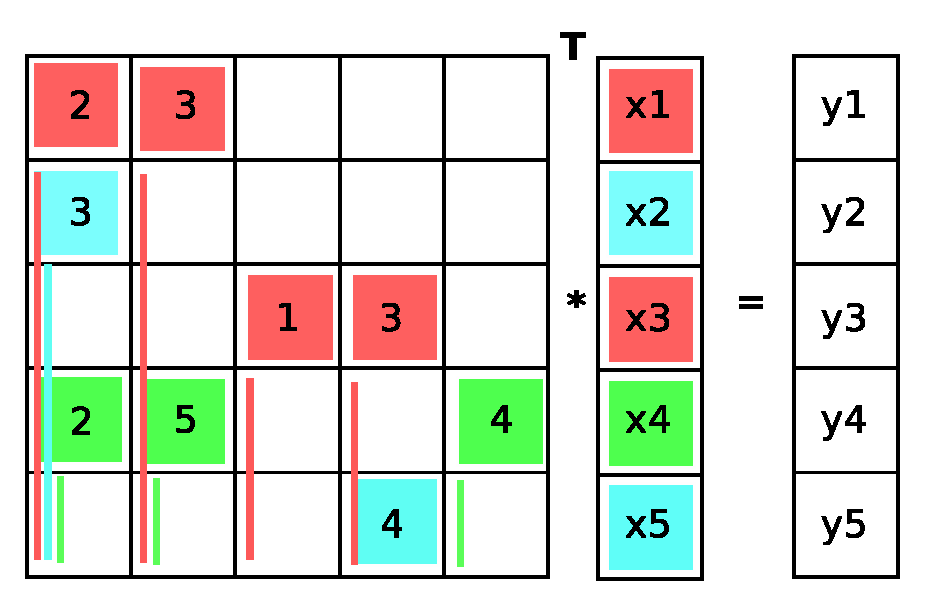
\includegraphics[width=0.32\textwidth]{graphic/coloringT10.eps}
\caption{Coloring of a Simple Matrix}\label{figure:coloring}
\end{figure}

This is easy to perform for small matrices. To cope with larger matrices we
iterate through the matrix for every color and store the position of blocked
nonzero elements for the specific color in a mask.
Each row is compared to the mask and if no nonzero entry of the row interferes
with the already blocked entries, the row is added to the current color and the
mask gets updated accordingly.
As long as there are uncolored rows of the matrix new colors will be used.
To further optimize this we use a mask for 32 colors at once.

\lstset{language=C++, numbers=left, captionpos=b,
        caption={Coloring of a matrix for transposed vector multiplication}}
\begin{lstlisting}
void Coloring ()
  {
    int height = this->Height();
    int width = this->Width();

    Array<int> row_color(height);
    row_color = -1;

    int maxcolor = 0;
    int basecol = 0;

    Array<unsigned int> mask(width);

    int found = 0;

    do
    {
      mask = 0;

      for (int row = 0; row < height; ++row)
      {
        if (row_color[row] >= 0) continue;

        int first = firsti [row];
        int last  = firsti [row+1];

        unsigned check = 0;
        for (int i = first; i < last; ++i)
          check |= mask[colnr[i]];

        if (check != UINT_MAX)
        {
          found++;
          unsigned checkbit = 1;
          int color = basecol;
          while (check & checkbit)
          {
            color++;
            checkbit *= 2;
          }

          row_color[row] = color;
          if (color > maxcolor) maxcolor = color;

          for (int i = first; i < last; ++i)
            mask[colnr[i]] |= checkbit;
        }
      }

      basecol += 8*sizeof(unsigned int); // 32;
    }
    while (found < height);

    Array<int> cntcol(maxcolor+1);
    cntcol = 0;
    for (int row = 0; row < height; ++row)
      ++cntcol[row_color[row]];

    coloring_ = table<int>(cntcol);

    cntcol = 0;
    for (int row = 0; row < height; ++row)
      coloring_[row_color[row]][cntcol[row_color[row]]++] = row;

    std::cout << "needed " << maxcolor+1 << " colors" << std::endl;
  }

\end{lstlisting}

\lstset{language=c++, numbers=left, captionpos=b,
        caption={transposed vector multiplication by coloring a matrix}}
\begin{lstlisting}
void TranMultAdd4 (double s, const BaseVector & x, BaseVector & y)
  {
    FlatVector<double> fx = x.FV<double> ();
    FlatVector<double> fy = y.FV<double> ();

    Coloring();

#pragma omp parallel
    {
      for (auto color : coloring_)
      {
#pragma omp for
        for (int i = 0; i < color.Size(); ++i)
        {
          int first = firsti [color[i]];
          int last  = firsti [color[i]+1];

          for (int j = first; j < last; ++j)
          {
            fy(colnr[j]) += s * data[j] * fx(color[i]);
          }
        }
      }
    }
  }


\end{lstlisting}

\section{Gauß-Seidel Method}
As mentioned in chapter~\ref{section:motiv} we use two Gauß-Seidel steps on
each level. The Gauß-Seidel method is similar to the Jacobi method.
Both methods need to compute the vector $Ax$. The difference is, that the
Gauß-Seidel method also uses the new information obtained by previous
computations of entries.
In particular a new entry is given by:
$$ x_j^{new} = \frac{1}{A_{jj}} \left(b_{j} - \sum_{k \in K^{new}}A_{jk}
x_k^{new} - \sum_{k \in K^{old}}A_{jk} x_k^{old}\right) \qquad j = 1 \dots n$$
$K^{new}$ denotes the index set of newly calculated entries
of $x$ and $K^{old}$ denotes the index set of old entries.
\cite{numerik} \cite{numpde}

The calculation order in the forward Gauß-Seidel precondition is arbitrary,
but to achieve a symmetric preconditioner the backward smoothing needs to be
in exact reverse order.

Entries of the output vector $x$ must not be calculated concurrently if they
depend on each other. As in chapter~\ref{section:trans} described, this would
cause incorrect entries. The problems with parallelization are also very
similar to chapter~\ref{section:trans}, as are the ideas to cope with them.

A coloring algorithm can be used as well and is similar in its implementation.
As with the transposed matrix vector multiplication we group the rows which
may run parallel without influencing each other.

\subsection{Coloring}
To calculate the product $A_jx$ which modifies the entry $x_j$ (where $A_j$
denotes the j-th row of the matrix $A$), for every $k$ with $A_{jk} \neq 0$,
$x_k$ is used. According to this observation, every row $A_j$, which should be
added to an existing color has to have zero elements on the positions $A_{jk}$
for all $k$ indices of rows marked with this color.?????

Instead of testing all remaining rows for this property, we use that $A$ is
symmetric: $A_{kj} = 0 \Leftrightarrow A_{jk} = 0$. Thus we only check
the specific row we added to one color to determine which rows can also
relate to it.

The main advantage of this method is, that the coloring process has to be
done only once, whereas it is used by GSSmooth and GSSmoothBack as well.
Also the order of colors is stored by the process itself.

For a small matrix the coloring process is demonstrated in
figure~\ref{figure:coloringGS}.

\begin{figure}
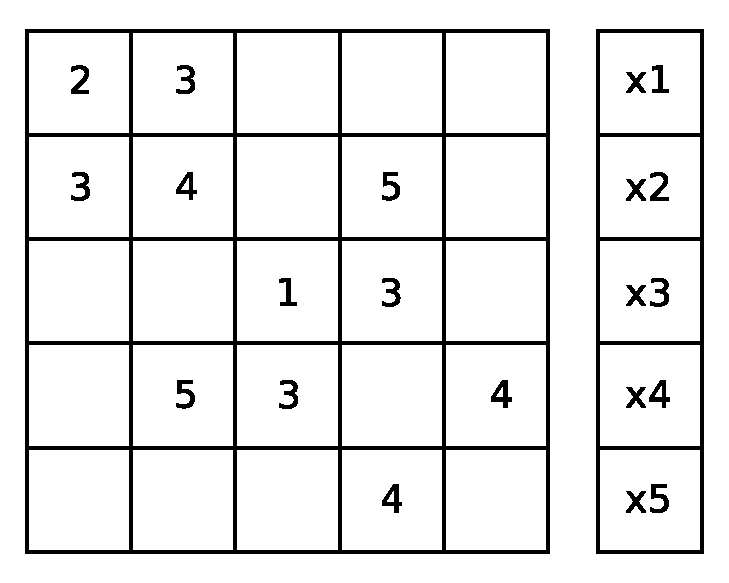
\includegraphics[width=0.32\textwidth]{graphic/coloringGS1.eps}\hfill\vline\hfill
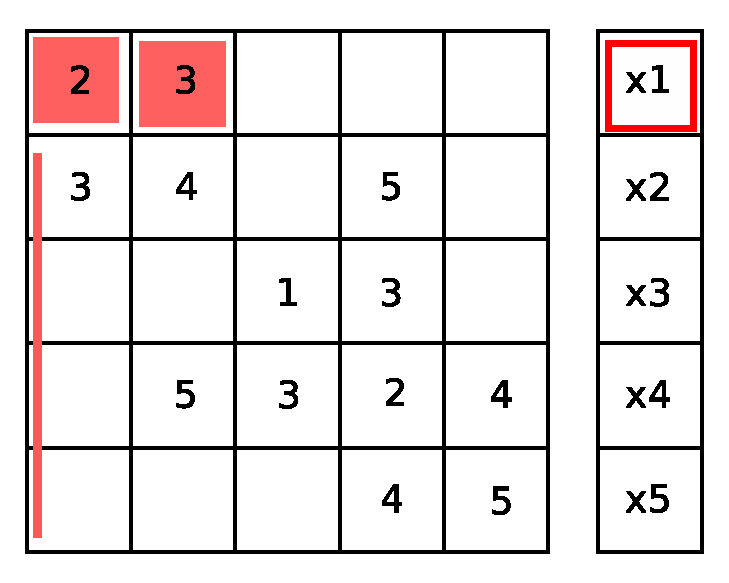
\includegraphics[width=0.32\textwidth]{graphic/coloringGS4.eps}\hfill\vline\hfill
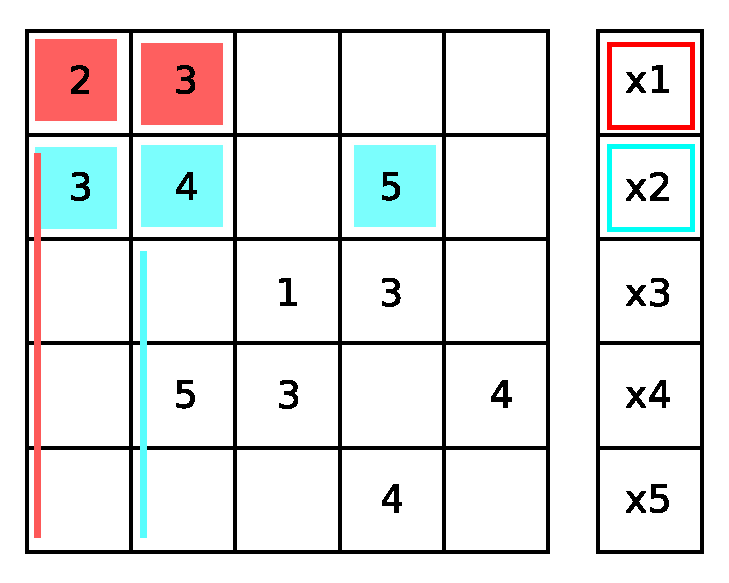
\includegraphics[width=0.32\textwidth]{graphic/coloringGS7.eps}
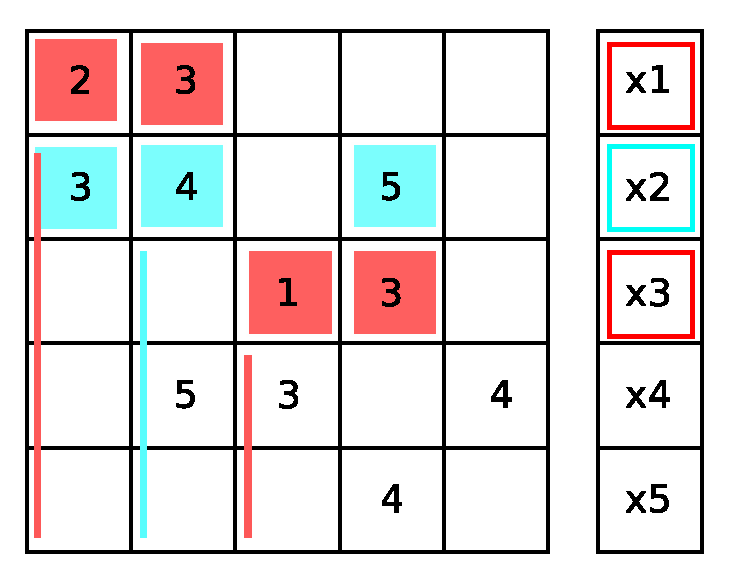
\includegraphics[width=0.32\textwidth]{graphic/coloringGS8.eps}\hfill\vline\hfill
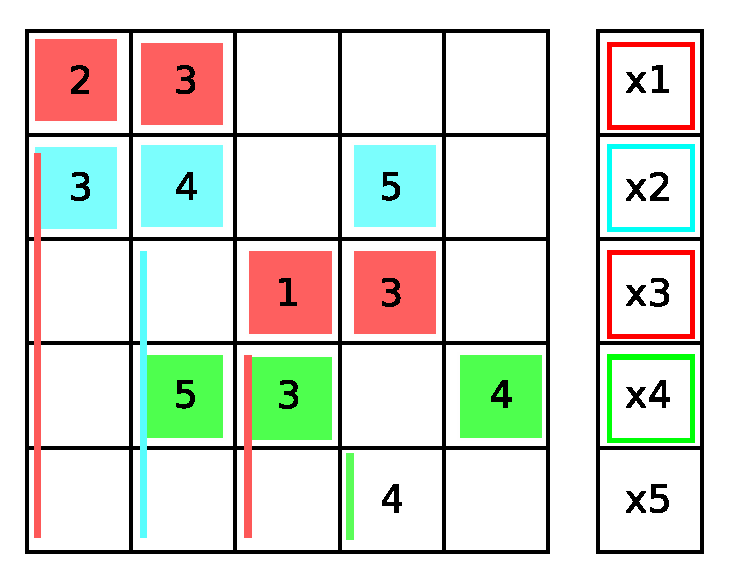
\includegraphics[width=0.32\textwidth]{graphic/coloringGS9.eps}\hfill\vline\hfill
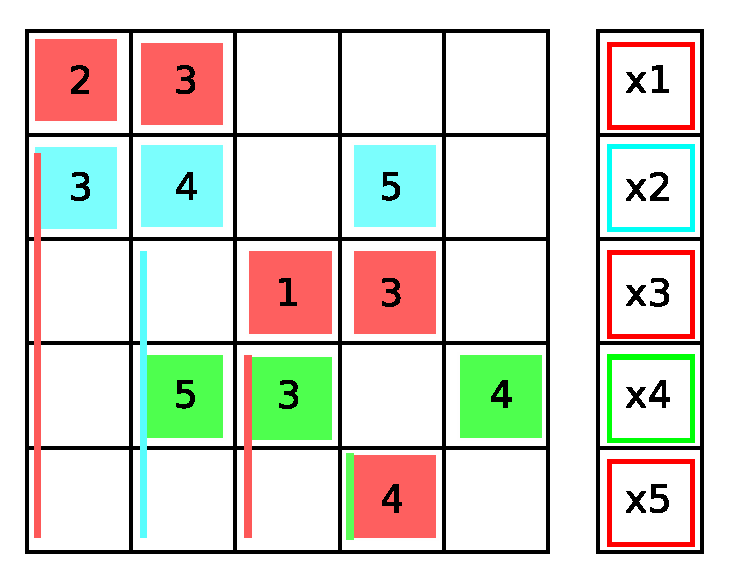
\includegraphics[width=0.32\textwidth]{graphic/coloringGS10.eps}
\caption{Coloring of a simple matrix.}\label{figure:coloringGS}
\end{figure}

\subsection{Speed Improvement}
As mentioned, the AMG preconditioner is a combination of the Gauß-Seidel
preconditioner and intermediate projections onto coarser spaces
by multiplying with the transposed prolongation matrix. These steps are
executed alternately until the matrix is small enough to invert it directly.
Then the correction is refined to its original size and backwards Gauß-Seidel is
used in between these steps.
This sums up to one step of the AMG-Preconditioner. Many of such steps are
executed in succession until the solution is sufficiently exact.

Speed improvements by parallelization are possible within Gauß-Seidel steps
and the transposed matrix vector multiplication. The Gauß-Seidel coloring has to
be done separately for each level before the CG method, but can be used again
in each CG iteration. For the transposed matrix vector multiplication a
balancing algorithm is used.

Figure~\ref{figure:sequ} shows a CG method with sequential AMG, whereas
figure~\ref{figure:par} shows it with parallel AMG\@.
Only one thread is working in the sequential version compared to 24 threads in
the parallel.

In figure~\ref{figure:par} and~\ref{figure:step} the red blocks indicate a
thread of forward Gauß-Seidel smoothing, the purple ones are projections and
prolongations and the green ones indicate backward Gauß-Seidel smoothing.
In figure~\ref{figure:step} a single step of the AMG is shown. The large matrix
needs more time to perform a Gauß-Seidel step.
This is indicated by the big red blocks at the beginning. Only one color is
calculated at the same time, but its rows can be processed by several threads
simultaneously.

\begin{figure}
    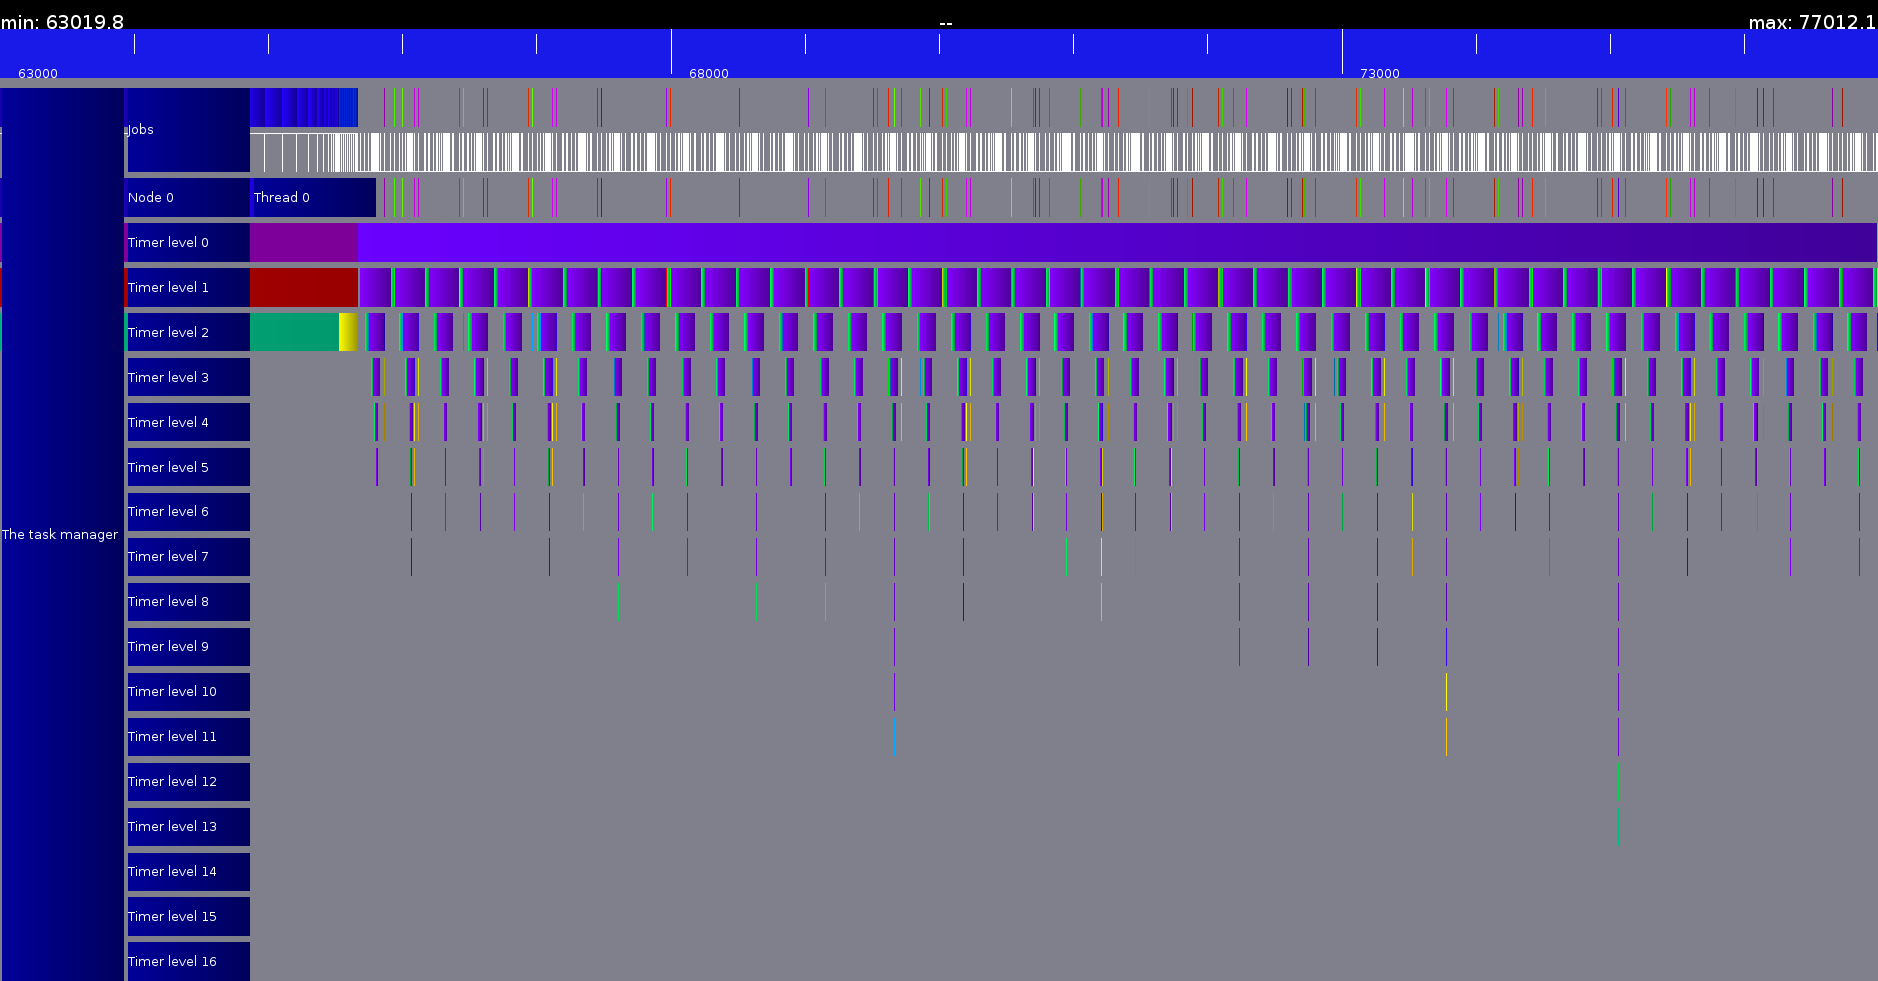
\includegraphics[width=1\textwidth]{seq.png}
    \caption{AMG sequential}\label{figure:sequ}
\end{figure}

\begin{figure}
    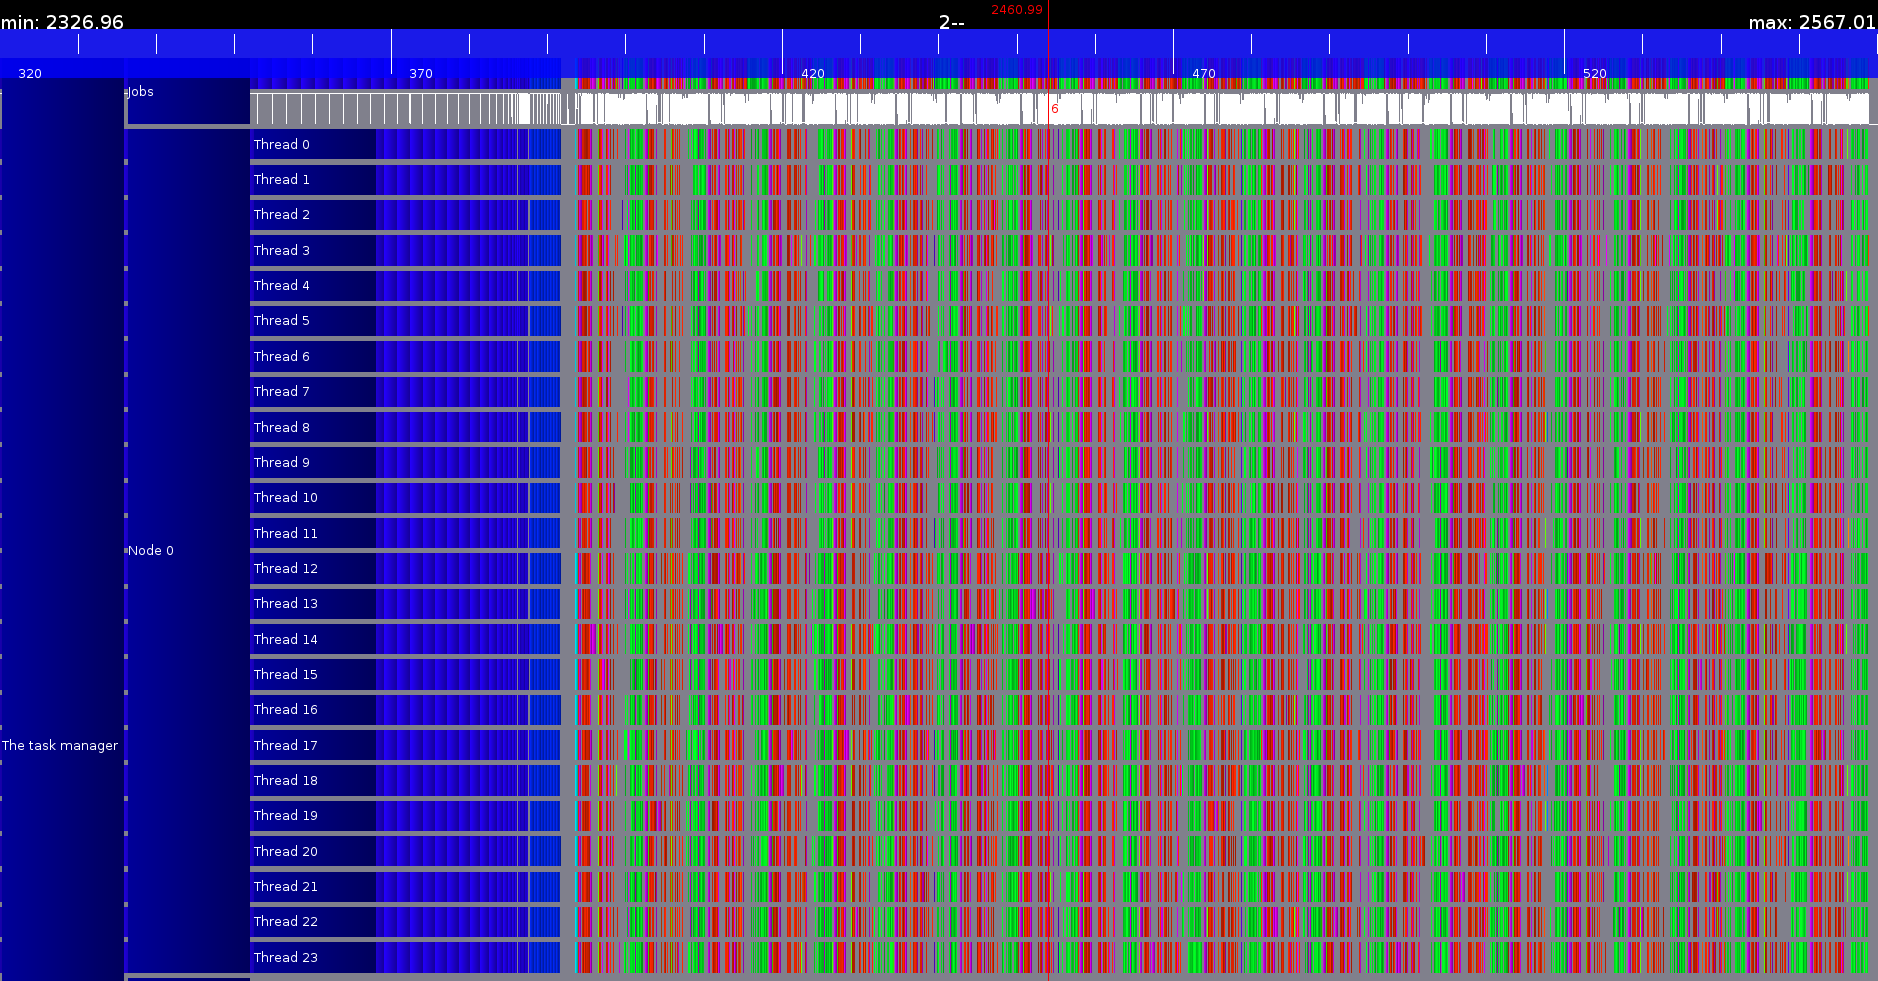
\includegraphics[width=1\textwidth]{iterations_trace.png}
    \caption{AMG parallel}\label{figure:par}
\end{figure}

\begin{figure}
    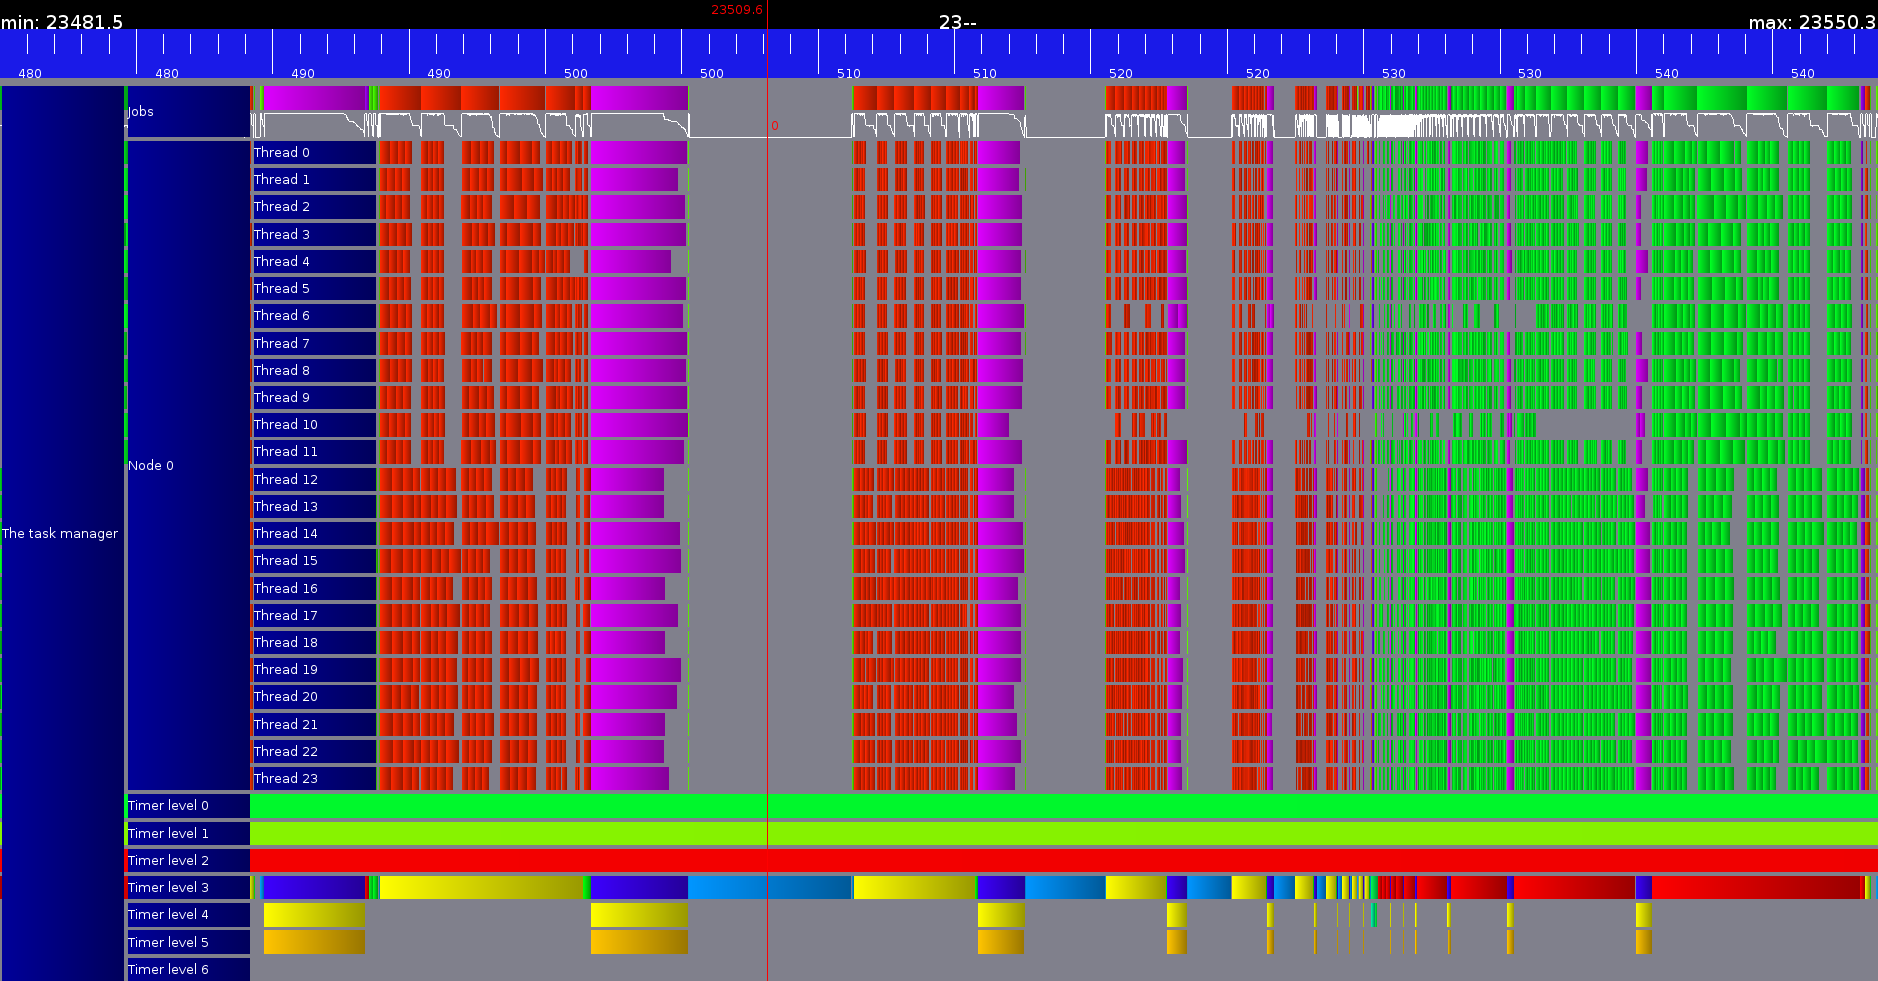
\includegraphics[width=1\textwidth]{undistributed_coloring_gs.png}
    \caption{AMG single parallel recursion}\label{figure:step}
\end{figure}

Due to the matrix storage and the specific structure of the {\em Vector}\/
server its two processors have different speed of writing and reading at parts
of the matrix. Due to this some colors are faster calculated by the first half
of threads, and others by the other half. This comes up with the coloring process. Iteration through the matrix will color
most of the first rows with the first colors and vice versa.

A comparison of figure \ref{figure:step} and figure \ref{figure:stepdis} shows
that most of the gray spaces between the blocks can be eliminated by minimizing the
correspondence of rows and colors.

\begin{figure}
    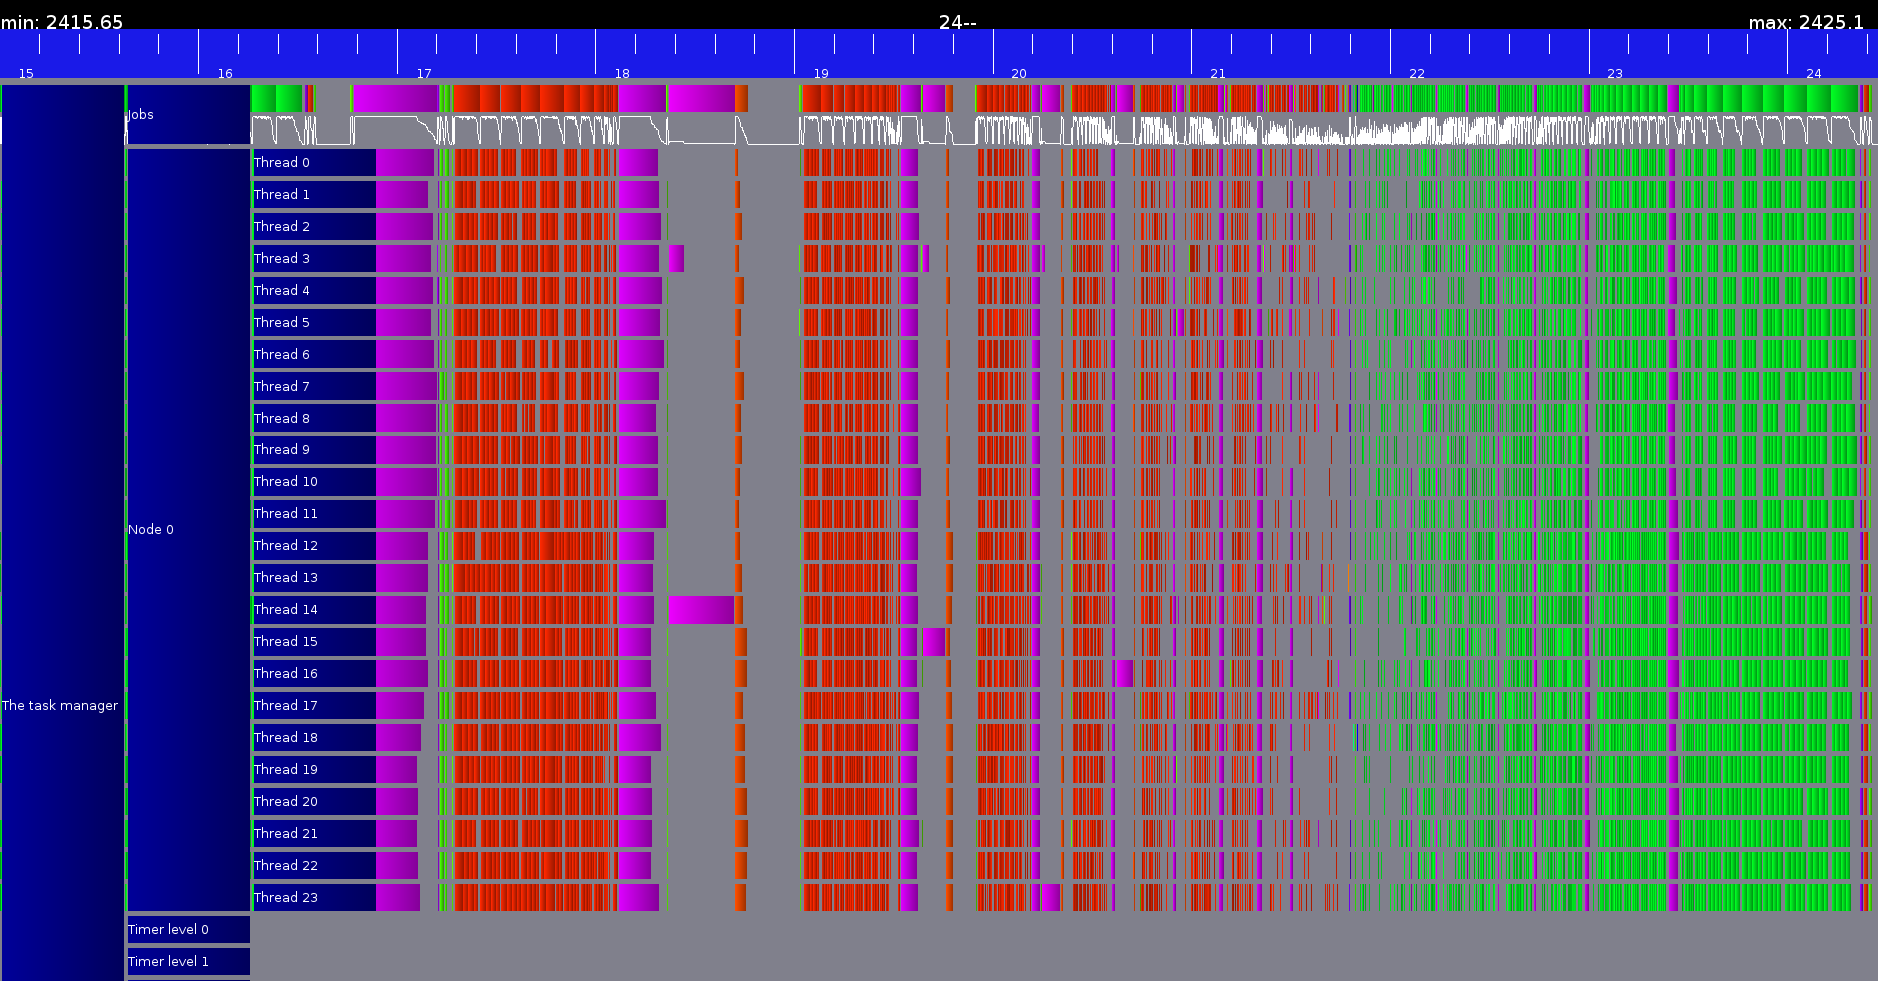
\includegraphics[width=1\textwidth]{one_iteration.png}
    \caption{AMG single parallel recursion with distribution}\label{figure:stepdis}
\end{figure}

\pagebreak

\section{Code}


\lstset{language=C++, numbers=left, captionpos=b, breaklines=true,
        caption={Multiplication Method of the AMG Preconditioner}}
\begin{lstlisting}
void my_AMG_H1 :: Mult (const ngla::BaseVector & b, ngla::BaseVector & x) const {
  if (inv) {
    x = (*inv) * b;
    return;
  }

  auto residuum = pmat->CreateVector();
  auto coarse_x = coarsemat->CreateVector();
  auto coarse_residuum = coarsemat->CreateVector();

  x = 0;
  jacobi->GSSmooth (x, b);

  if (recAMG) {
    residuum = b - (*pmat) * x;
    coarse_residuum = ngla::Transpose (*prol) * residuum;

    recAMG->Mult(coarse_residuum, coarse_x);

    x += (*prol) * coarse_x;
  }

  jacobi->GSSmoothBack (x, b);
}
\end{lstlisting}

\label{lst:mult}
\begin{figure}
%% Generated with LaTeXDraw 2.0.8
% Sun Jun 14 10:48:06 CEST 2015
% \usepackage[usenames,dvipsnames]{pstricks}
% \usepackage{epsfig}
% \usepackage{pst-grad} % For gradients
% \usepackage{pst-plot} % For axes
\scalebox{1} % Change this value to rescale the drawing.
{
\begin{pspicture}(0,-2.54)(6.48,2.54)
\definecolor{color641b}{rgb}{0.4823529411764706,0.996078431372549,0.9921568627450981}
\definecolor{color641}{rgb}{0.996078431372549,0.996078431372549,0.996078431372549}
\definecolor{color644b}{rgb}{0.996078431372549,0.37254901960784315,0.37254901960784315}
\definecolor{color651b}{rgb}{0.3058823529411765,1.0,0.3058823529411765}
\definecolor{color661c}{rgb}{0.5019607843137255,0.5019607843137255,0.5019607843137255}
\definecolor{color713}{rgb}{0.9921568627450981,0.34509803921568627,0.34509803921568627}
\definecolor{color715}{rgb}{0.34509803921568627,0.9921568627450981,0.9921568627450981}
\definecolor{color716}{rgb}{0.3568627450980392,0.9921568627450981,0.34509803921568627}
\psframe[linewidth=0.02,linecolor=color641,dimen=outer,fillstyle=solid,fillcolor=color641b](0.83,1.39)(0.07,0.63)
\psframe[linewidth=0.02,linecolor=color641,dimen=outer,fillstyle=solid,fillcolor=color641b](1.85,1.41)(1.09,0.65)
\psframe[linewidth=0.02,linecolor=color641,dimen=outer,fillstyle=solid,fillcolor=color641b](3.89,1.41)(3.13,0.65)
\psframe[linewidth=0.02,linecolor=color641,dimen=outer,fillstyle=solid,fillcolor=color644b](2.89,0.39)(2.13,-0.37)
\psframe[linewidth=0.02,linecolor=color641,dimen=outer,fillstyle=solid,fillcolor=color644b](3.89,0.39)(3.13,-0.37)
\usefont{T1}{ppl}{m}{n}
\rput(3.4664063,-0.03){3}
\psframe[linewidth=0.02,linecolor=color641,dimen=outer,fillstyle=solid,fillcolor=color641b](6.35,1.39)(5.59,0.63)
\psframe[linewidth=0.02,linecolor=color641,dimen=outer,fillstyle=solid,fillcolor=color644b](6.35,0.37)(5.59,-0.39)
\psframe[linewidth=0.02,linecolor=color641,dimen=outer,fillstyle=solid,fillcolor=color651b](1.85,-0.61)(1.09,-1.37)
\psframe[linewidth=0.02,linecolor=color641,dimen=outer,fillstyle=solid,fillcolor=color651b](2.89,-0.63)(2.13,-1.39)
\psframe[linewidth=0.02,linecolor=color641,dimen=outer,fillstyle=solid,fillcolor=color651b](4.91,-0.61)(4.15,-1.37)
\psframe[linewidth=0.02,linecolor=color641,dimen=outer,fillstyle=solid,fillcolor=color651b](6.35,-0.63)(5.59,-1.39)
\psframe[linewidth=0.02,linecolor=color641,dimen=outer,fillstyle=solid,fillcolor=color644b](6.35,-1.63)(5.59,-2.39)
\psframe[linewidth=0.02,linecolor=color641,dimen=outer,fillstyle=solid,fillcolor=color644b](3.89,-1.57)(3.13,-2.33)
\psframe[linewidth=0.02,linecolor=color641,dimen=outer,fillstyle=solid,fillcolor=color644b](6.35,2.37)(5.59,1.61)
\psframe[linewidth=0.02,linecolor=color641,dimen=outer,fillstyle=solid,fillcolor=color644b](0.83,2.43)(0.07,1.67)
\psframe[linewidth=0.02,linecolor=color641,dimen=outer,fillstyle=solid,fillcolor=color644b](1.85,2.39)(1.09,1.63)
\rput(0.0,-2.5){\psgrid[gridwidth=0.028222222,subgridwidth=0.014111111,gridlabels=0.0pt,subgridcolor=color661c](0,0)(0,0)(5,5)}
\usefont{T1}{ppl}{m}{n}
\rput(0.4846875,2.01){2}
\usefont{T1}{ppl}{m}{n}
\rput(1.4964062,2.01){3}
\usefont{T1}{ppl}{m}{n}
\rput(1.515625,0.99){4}
\usefont{T1}{ppl}{m}{n}
\rput(2.4659376,-0.0253125){1}
\usefont{T1}{ppl}{m}{n}
\rput(4.535625,-1.0053124){4}
\usefont{T1}{ppl}{m}{n}
\rput(1.4945313,-1.0053124){5}
\usefont{T1}{ppl}{m}{n}
\rput(3.485625,-2.01){4}
\usefont{T1}{ppl}{m}{n}
\rput(2.4864063,-1.01){3}
\usefont{T1}{ppl}{m}{n}
\rput(0.48640624,0.9853125){3}
\usefont{T1}{ppl}{m}{n}
\rput(3.4645312,0.99){5}
\rput(5.48,-2.5){\psgrid[gridwidth=0.028222222,subgridwidth=0.014111111,gridlabels=0.0pt,subgridcolor=color661c](0,0)(0,0)(1,5)}
\usefont{T1}{ppl}{m}{n}
\rput(5.9428124,2.0146875){x1}
\usefont{T1}{ppl}{m}{n}
\rput(5.9414062,0.9853125){x2}
\usefont{T1}{ppl}{m}{n}
\rput(5.945,-0.03){x3}
\usefont{T1}{ppl}{m}{n}
\rput(5.9492188,-1.0053124){x4}
\usefont{T1}{ppl}{m}{n}
\rput(5.943594,-2.01){x5}
\psline[linewidth=0.06cm,linecolor=color713](0.1,1.32)(0.1,-2.36)
\psline[linewidth=0.06cm,linecolor=color713](2.12,-0.62)(2.12,-2.36)
\psline[linewidth=0.06cm,linecolor=color715](1.12,0.38)(1.12,-2.36)
\psline[linewidth=0.06cm,linecolor=color716](3.1,-1.56)(3.1,-2.38)
\end{pspicture} 
}



\end{figure}

\lstset{language=c++, numbers=left, captionpos=b,
        caption={Gauß-Seidel coloring and balancing}}
\begin{lstlisting}

  void JacobiPrecond<TM,TV_ROW,TV_COL> :: Coloring ()
  {
    //static Timer timer("JacobiPrecond::Coloring");
    //RegionTimer reg (timer);

    int height = mat.Height();
    int width = mat.Width();

    Array<int> row_color(height);
    row_color = -1;

    int maxcolor = 0;
    int basecol = 0;

    Array<unsigned int> mask(width);

    int found = 0;

    int num_threads = task_manager->GetNumThreads();

    do
    {
      mask = 0;

      int block_size = ceil((double)height / (double)num_threads);

      for (int block_row = 0; block_row < block_size; ++block_row)
      {
        for (int threadi = 0; threadi < num_threads; ++threadi)
        {
          int row = block_row + threadi * block_size;
          if (row >= height) break;
          if (row_color[row] >= 0) continue;

          int first = mat.firsti [row];
          int last  = mat.firsti [row+1];

          unsigned check = 0;
          for (int i = first; i < last; ++i)
            check |= mask[mat.colnr[i]];

          if (check != UINT_MAX) // 0xFFFFFFFF)
          {
            found++;
            unsigned checkbit = 1;
            int color = basecol;
            while (check & checkbit)
            {
              color++;
              checkbit *= 2;
            }

            row_color[row] = color;
            if (color > maxcolor) maxcolor = color;

            mask[row] |= checkbit;
          }
        }
      }

      basecol += 8*sizeof(unsigned int); // 32;
    }
    while (found < height);

    Array<int> cntcol(maxcolor+1);
    cntcol = 0;
    for (int row = 0; row < height; ++row)
      ++cntcol[row_color[row]];

    coloring_ = Table<int>(cntcol);

    cntcol = 0;
    for (int row = 0; row < height; ++row)
      coloring_[row_color[row]][cntcol[row_color[row]]++] = row;

    balancing_.SetSize (maxcolor+1);
    for (auto c : Range (balancing_))
    {
      balancing_[c].Calc (coloring_[c].Size(),
        [&] (int bi)
        {
          return 5 + mat.GetRowIndices(coloring_[c][bi]).Size();
        });
    }

    //cout << "Balancing: " << balancing_ << endl;
    std::cout << "needed " << maxcolor+1 << " colors" << std::endl;
  }

\end{lstlisting}

\lstset{language=c++, numbers=left, captionpos=b,
        caption={Gauß-Seidel Smooth}}
\begin{lstlisting}



  void JacobiPrecond<TM,TV_ROW,TV_COL> ::
  GSSmooth (BaseVector & x, const BaseVector & b) const
  {
    //static Timer timer("JacobiPrecond::GSSmooth");
    //timer.AddFlops (mat.NZE());
    //RegionTimer reg (timer);

    FlatVector<TV_ROW> fx = x.FV<TV_ROW> ();
    // dynamic_cast<T_BaseVector<TV_ROW> &> (x).FV();
    const FlatVector<TV_ROW> fb = b.FV<TV_ROW> ();
    // dynamic_cast<const T_BaseVector<TV_ROW> &> (b).FV();

    for (int j = 0; j < this->coloring_.Size(); ++j)
    {
      auto color = this->coloring_[j];
      ParallelFor( this->balancing_[j],
        [this, fx, fb, color] (int i)
        {
          int row = color[i];
          if (!this->inner || this->inner->Test(row))
          {
            TV_ROW ax = mat.RowTimesVector (row, fx);
            fx(row) += invdiag[row] * (fb(row) - ax);
          }
        }, 4);
    }
  }
\end{lstlisting}

\lstset{language=c++, numbers=left, captionpos=b,
        caption={Gauß-Seidel SmoothBack}}
\begin{lstlisting}
  void JacobiPrecond<TM,TV_ROW,TV_COL> ::
  GSSmoothBack (BaseVector & x, const BaseVector & b) const
  {
    //static Timer timer("JacobiPrecond::GSSmoothBack");
    //timer.AddFlops (mat.NZE());
    //RegionTimer reg (timer);

    FlatVector<TV_ROW> fx = x.FV<TV_ROW> ();
    // dynamic_cast<T_BaseVector<TV_ROW> &> (x).FV();
    const FlatVector<TV_ROW> fb = b.FV<TV_ROW> ();
    //dynamic_cast<const T_BaseVector<TV_ROW> &> (b).FV();

    for (int j = this->coloring_.Size()-1; j >= 0; --j)
    {
      auto color = this->coloring_[j];
      ParallelFor( this->balancing_[j],
        [this, fx, fb, color] (int i)
        {
          int row = color[i];
          if (!this->inner || this->inner->Test(row))
          {
            TV_ROW ax = mat.RowTimesVector (row, fx);
            fx(row) += invdiag[row] * (fb(row) - ax);
          }
        }, 4);
    }
  }


\end{lstlisting}



\bibliography{doc}{}
\bibliographystyle{plain}
\end{document}
